\documentclass{article}

\usepackage[final]{style}
\usepackage[utf8]{inputenc}
\usepackage[brazilian]{babel}
\usepackage[T1]{fontenc}
\usepackage{hyperref}
\usepackage{url}
\usepackage{booktabs}
\usepackage{amsfonts}
\usepackage{microtype}
\usepackage{xcolor}
\usepackage{graphicx}
\graphicspath{{../output/}}
\usepackage{listings}
\usepackage{multicol}
\usepackage{amsmath}
\usepackage[font=footnotesize]{caption}
\DeclareMathOperator*{\argmin}{arg\!min}
\usepackage{subcaption}
\definecolor{blue}{RGB}{41,5,195}
\makeatletter
\hypersetup{colorlinks=true,linkcolor=blue,citecolor=red,urlcolor=blue}
\makeatother

\renewcommand{\figureautorefname}{Figura}
\newcommand{\media}[1]{\ensuremath{\bar{#1\vphantom{+1}}}}

\title{Relatório\\Primeira Lista de Exercícios}

\author{
  Rodrigo Ferreira Berriel\\
  LCAD @ UFES
}


\begin{document}

\maketitle

\begin{abstract}
  Esse relatório visa apresentar os resultados alcançados com a primeira lista de exercícios, bem como responder as questões feitas em cada exercício. Além desse relatório, foi enviado o código-fonte para a reprodução dos resultados apresentados nesse relatório. O código-fonte também se encontra disponível no GitHub:
  
  \url{http://github.com/rodrigoberriel/aprendizado-de-maquina-2017-1}
\end{abstract}

\section{Exercício 1}

Dada a base de dados \texttt{Iris} (disponibilizada em \url{http://archive.ics.uci.edu/ml/}), obtenha:

\paragraph{a)} A média e variância de cada um dos atributos:

Para cada atributo, a média e variância foram calculadas e apresentadas na \autoref{tab:ex1-a}.

\begin{table}[h]
	\centering
	\caption{Média e variância de cada atributo da base de dados Iris}
	\label{tab:ex1-a}
	\begin{tabular}{@{}ccc@{}}
		\toprule
		Atributo         & Média & Variância \\ \midrule
		sepal length     & 5.843 & 0.681     \\
		sepal width      & 3.054 & 0.187     \\
		petal length     & 3.759 & 3.092     \\
		petal width      & 1.199 & 0.579     \\ \bottomrule
	\end{tabular}
\end{table}



\paragraph{b)} A média e variância de cada um dos atributos para cada uma das classes:

Para cada classe, a média e a variância de cada um dos atributos foram calculadas e apresentadas na \autoref{tab:ex1-b-media} e \autoref{tab:ex1-b-variancia}, respectivamente.

\begin{table}[h]
	\centering
	\caption{Média de cada atributo para cada classe da base de dados Iris}
	\label{tab:ex1-b-media}
	\begin{tabular}{@{}lccc@{}}
		\toprule
		Atributo         & Iris-setosa & Iris-versicolor & Iris-virginica \\ \midrule
		sepal length     & 5.006       & 5.936           & 6.588          \\
		sepal width      & 3.418       & 2.770           & 2.974          \\
		petal length     & 1.464       & 4.260           & 5.552          \\
		petal width      & 0.244       & 1.326           & 2.026          \\ \bottomrule
	\end{tabular}
\end{table}

\begin{table}[h]
	\centering
	\caption{Variância de cada atributo para cada classe da base de dados Iris}
	\label{tab:ex1-b-variancia}
	\begin{tabular}{@{}lccc@{}}
		\toprule
		Atributo         & Iris-setosa & Iris-versicolor & Iris-virginica \\ \midrule
		sepal length     & 0.122       & 0.261           & 0.396          \\
		sepal width      & 0.142       & 0.097           & 0.102          \\
		petal length     & 0.030       & 0.216           & 0.298          \\
		petal width      & 0.011       & 0.038           & 0.074          \\ \bottomrule
	\end{tabular}
\end{table}

\paragraph{c)} O histograma com 16 bins de cada um dos atributos para cada uma das classes (gere um único gráfico de histograma de 16 bins, ou seja, dividido em 16 segmentos, para cada atributo diferenciando as classes, para mostrar como estão distribuídos os valores para diferentes classes):

Os histogramas podem ser vistos na \autoref{fig:exercicio1-c}.

\begin{figure}[h]
	\centering
	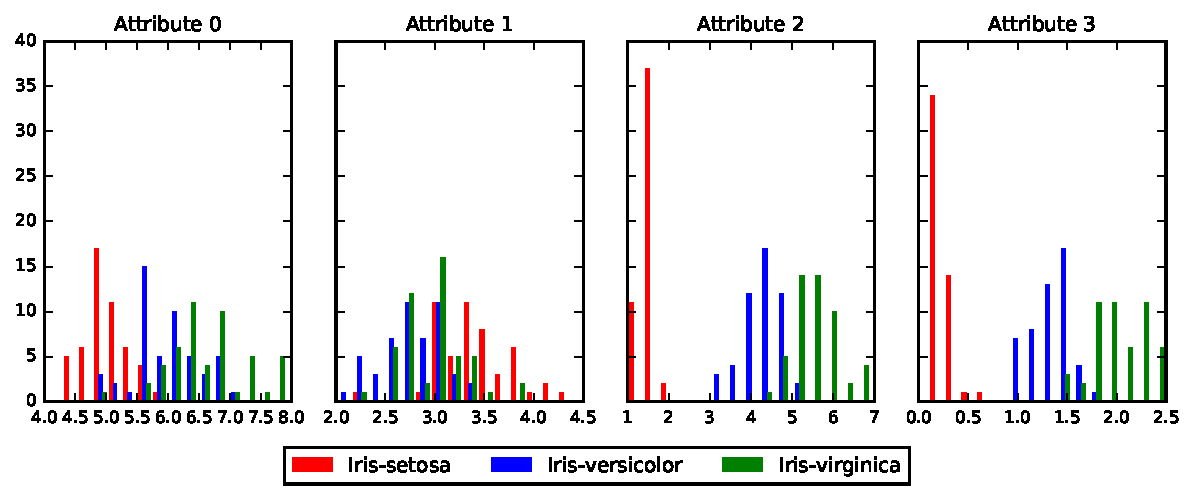
\includegraphics[width=\linewidth]{exercicio1-c.pdf}
	\caption{Histogramas de 16 bins para cada atributo diferenciando as classes por cores.}
	\label{fig:exercicio1-c}
\end{figure}


\paragraph{d)} Gere um gráfico 2D com os dois componentes principais (uso de PCA) das amostras, identificando cada classe. Pode usar a função \texttt{eig} do Matlab.

O gráfico, equivalente ao apresentado no Slide 21 da Aula 3, pode ser visto na \autoref{fig:exercicio1-d}.

\begin{figure}[h!]
	\centering
	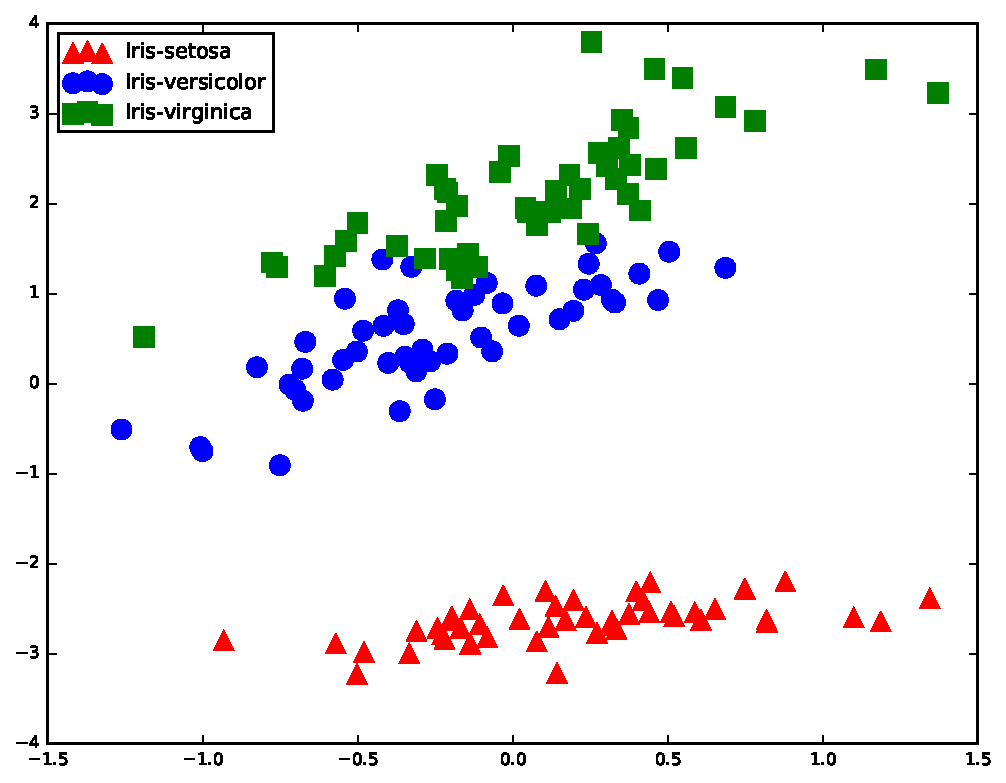
\includegraphics[width=0.5\linewidth]{exercicio1-d.pdf}
	\caption{Gráfico com as duas componentes principais.}
	\label{fig:exercicio1-d}
\end{figure}

\section{Exercício 2}

Dada a base de dados \texttt{CNAE-9\_reduzido} (em anexo):

\paragraph{a)} gere um gráfico 2D com os dois componentes principais (uso de PCA) das amostras, identificando cada classe (a base possui 5 classes. O rótulo das amostras está na primeira coluna. Essa coluna não deve ser usada no PCA).

Veja o gráfico na \autoref{fig:exercicio2-a}.

\begin{figure}[h]
	\centering
	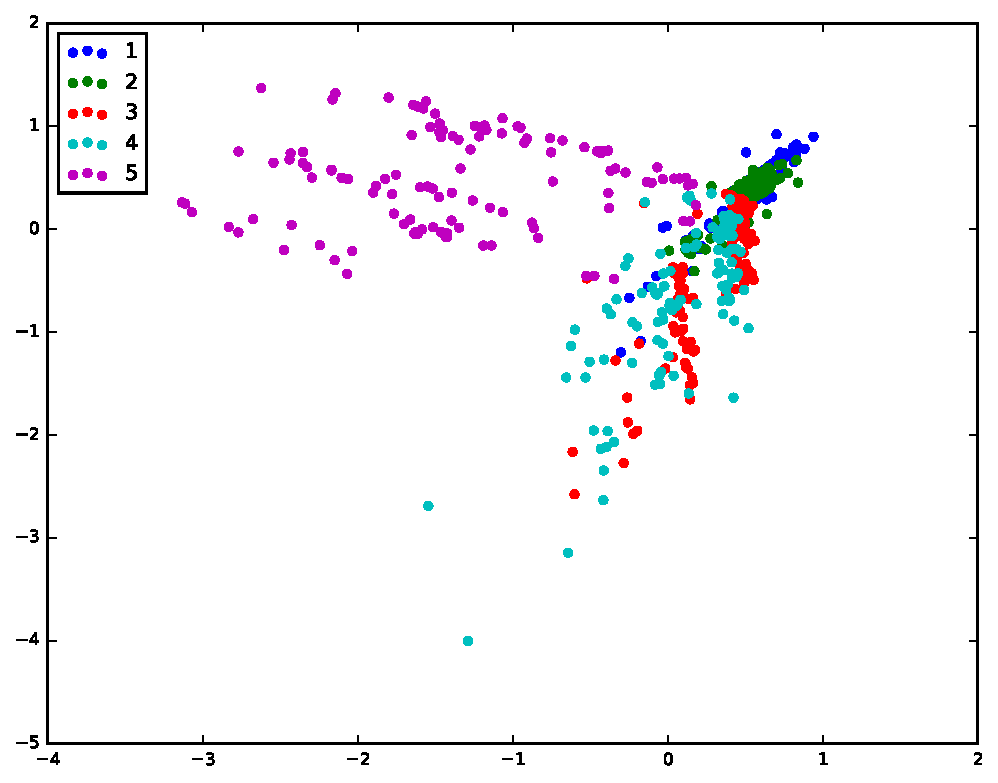
\includegraphics[width=0.5\linewidth]{exercicio2-a.pdf}
	\caption{Gráfico 2D com as duas componentes principais.}
	\label{fig:exercicio2-a}
\end{figure}

\paragraph{b)} gere um gráfico 2D com os dois componentes principais (uso de PCA) das amostras, identificando cada classe (a base possui 5 classes). Para este gráfico realize o branqueamento dos dados (isto é, após a aplicação do PCA garantir que a matriz de correlação dos dados seja uma matriz identidade). O que tem de diferente entre os gráficos de a) e b)?

Veja o gráfico na \autoref{fig:exercicio2-b}. O gráfico parece mais ``espalhado'' em comparação com a versão sem branqueamento, ou seja, os intervalos dos eixos aumentaram. Isso se deve ao fato do branqueamento garantir variância unitária, i.e., matriz de covariância igual a identidade.

\begin{figure}[h]
	\centering
	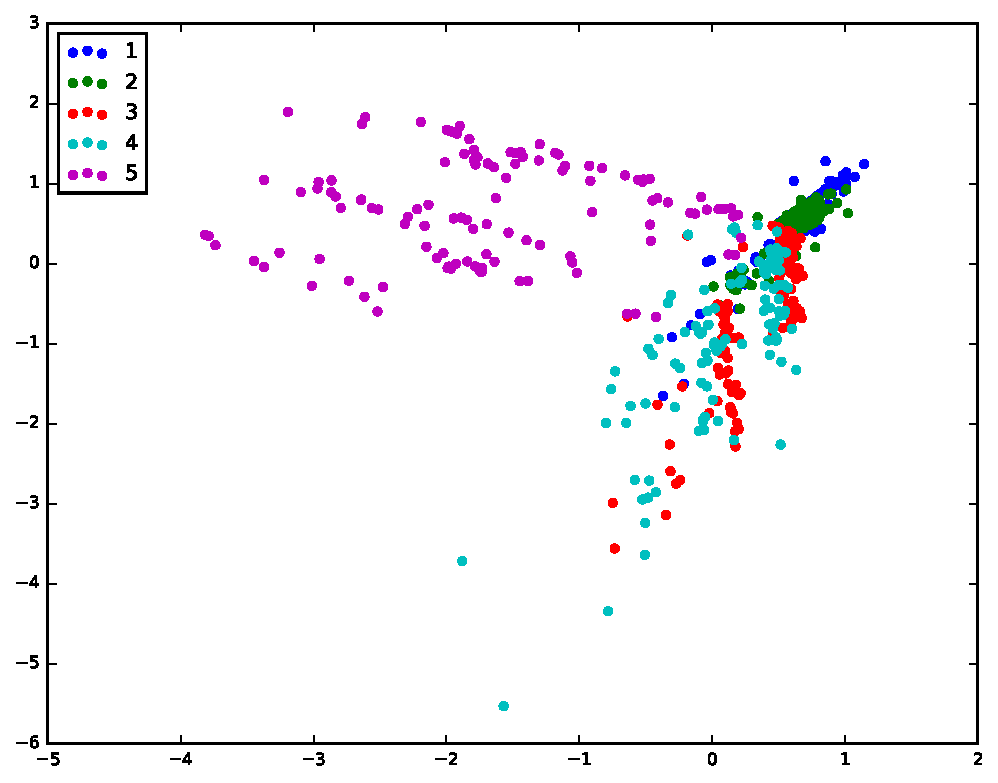
\includegraphics[width=0.5\linewidth]{exercicio2-b.pdf}
	\caption{Gráfico 2D com as duas componentes principais com branqueamento.}
	\label{fig:exercicio2-b}
\end{figure}

\paragraph{c)} Após a visualização dos gráficos, é possível identificar ao menos uma classe que possa ser facilmente separada das outras classes? Seria possível separar essa classe (sem grandes perdas) se fosse usada somente uma componente principal? Gere o gráfico de uma componente para explicar.

Pela \autoref{fig:exercicio2-b}, parece que as amostras da classe 5 podem ser facilmente separadas das demais. O gráfico 1D pode ser visto na \autoref{fig:exercicio2-c}, onde a classe 5 pode ser separada das demais com alguma perda usando somente uma componente principal. Como não há parâmetro do que seria uma ``grande perda'', eu diria que sim: a classe 5 pode ser separada das demais sem grandes perdas.

\begin{figure}[h]
	\centering
	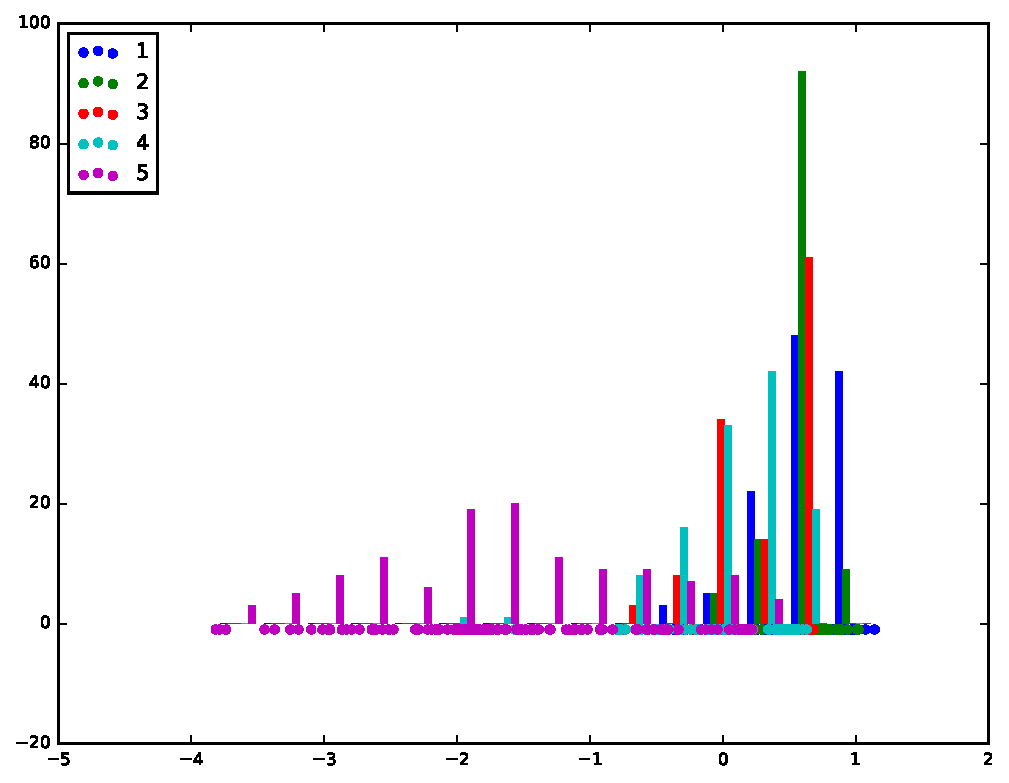
\includegraphics[width=0.5\linewidth]{exercicio2-c.pdf}
	\caption{Gráfico 1D com a componente principal com branqueamento. O histograma foi exibido acima do gráfico 1D para facilitar a visualização.}
	\label{fig:exercicio2-c}
\end{figure}

\section{Exercício 3}

A base de dados Nebulosa (disponibilizada em anexo) está contaminada com ruídos, redundâncias, dados incompletos, inconsistências e outliers. Para esta base:

\paragraph{a)} Obtenha os resultados da classificação (métrica acurácia) usando a técnica do vizinho mais próximo (NN) e Rocchio. Utilize a distância Euclidiana e a base de dados crua, sem pré-processamento. Use o conjunto de 143 amostras para treino e o de 28 amostras para teste. Proponha um tratamento para os dados incompletos.

Para tratar os dados incompletos (10 das 143 amostras de treino e 3 das 28 amostras de teste), foi usado o vizinho mais próximo. O valor incompleto de cada amostra foi substituído pelo valor do mesmo atributo do vizinho mais próximo. Para os dados de teste, a busca pelo vizinho mais próximo foi feita na base de treino. Com esses dados tratados, e usando toda a base de dados (menos a última coluna), os resultados de classificação (acurácia) alcançados foram:

\begin{itemize}
	\item NN: 50.000\%
	\item Rocchio: 50.000\%
\end{itemize}

\paragraph{b)} Realize um pré-processamento sobre os dados de forma a reduzir os ruídos, as redundâncias, inconsistências, outliers e a interferência dos dados incompletos. Obtenha os resultados da classificação usando a técnica do vizinho mais próximo (NN) e Rocchio usando a distância Euclidiana e a mesma divisão dos dados.

Para planejar o pré-processamento, foi visualizado o gráfico entre pares de atributos (\autoref{fig:exercicio3-a}). Como pode ser observado nesse gráfico, há diversos \textit{outliers}. Seguindo a orientação do Slide 65 da Aula 2, foram considerados \textit{outliers} todas as amostras que possuiam pelo menos 1 atributo com valor distantes mais de $x$ vezes o desvio padrão da média. Essa verificação foi feita iterativamente (com $x = (2 + (i\times0.5)))$, onde $i$ é o número da iteração), até que não fossem identificados outliers na base. Com esse processo de removação de \textit{outliers}, foram removidas 22 amostras, no total (18 na primeira iteração e 4 na segunda iteração). Como pode ser visto na \autoref{fig:exercicio3-a}, fica claro que 5 e 6 são atributos redundantes. Dessa forma, o atributo 6 foi removido da base de dados. Analisando os dados mais de perto, pode-se observar que existem algumas amostras duplicadas. Essas amostras (4, no total) foram removidas da base de treino. Além de amostras duplicadas, haviam outras amostras ambíguas, i.e., que possuíam todos os atributos idênticos mas classes diferentes. Para desambiguar essas amostras, a classe de cada uma delas foi definida como a do centróide mais próximo. No total, haviam 11 amostras ambíguas (5 únicas), fazendo com que 6 amostras fossem removidas da base de treino. Em todos os casos em que foi usada alguma medida de distância nas operações de pré-processamento, a medida foi a distância Euclidiana. Os dois primeiros atributos são identificadores dos usuários, portanto foram desconsiderados durante o treino. Depois das operações de pré-processamento (\autoref{fig:exercicio3-b}), a base de treino ficou com 111 amostras.

\begin{figure*}[h!]
	\centering
	\begin{subfigure}[t]{0.49\textwidth}
		\centering
		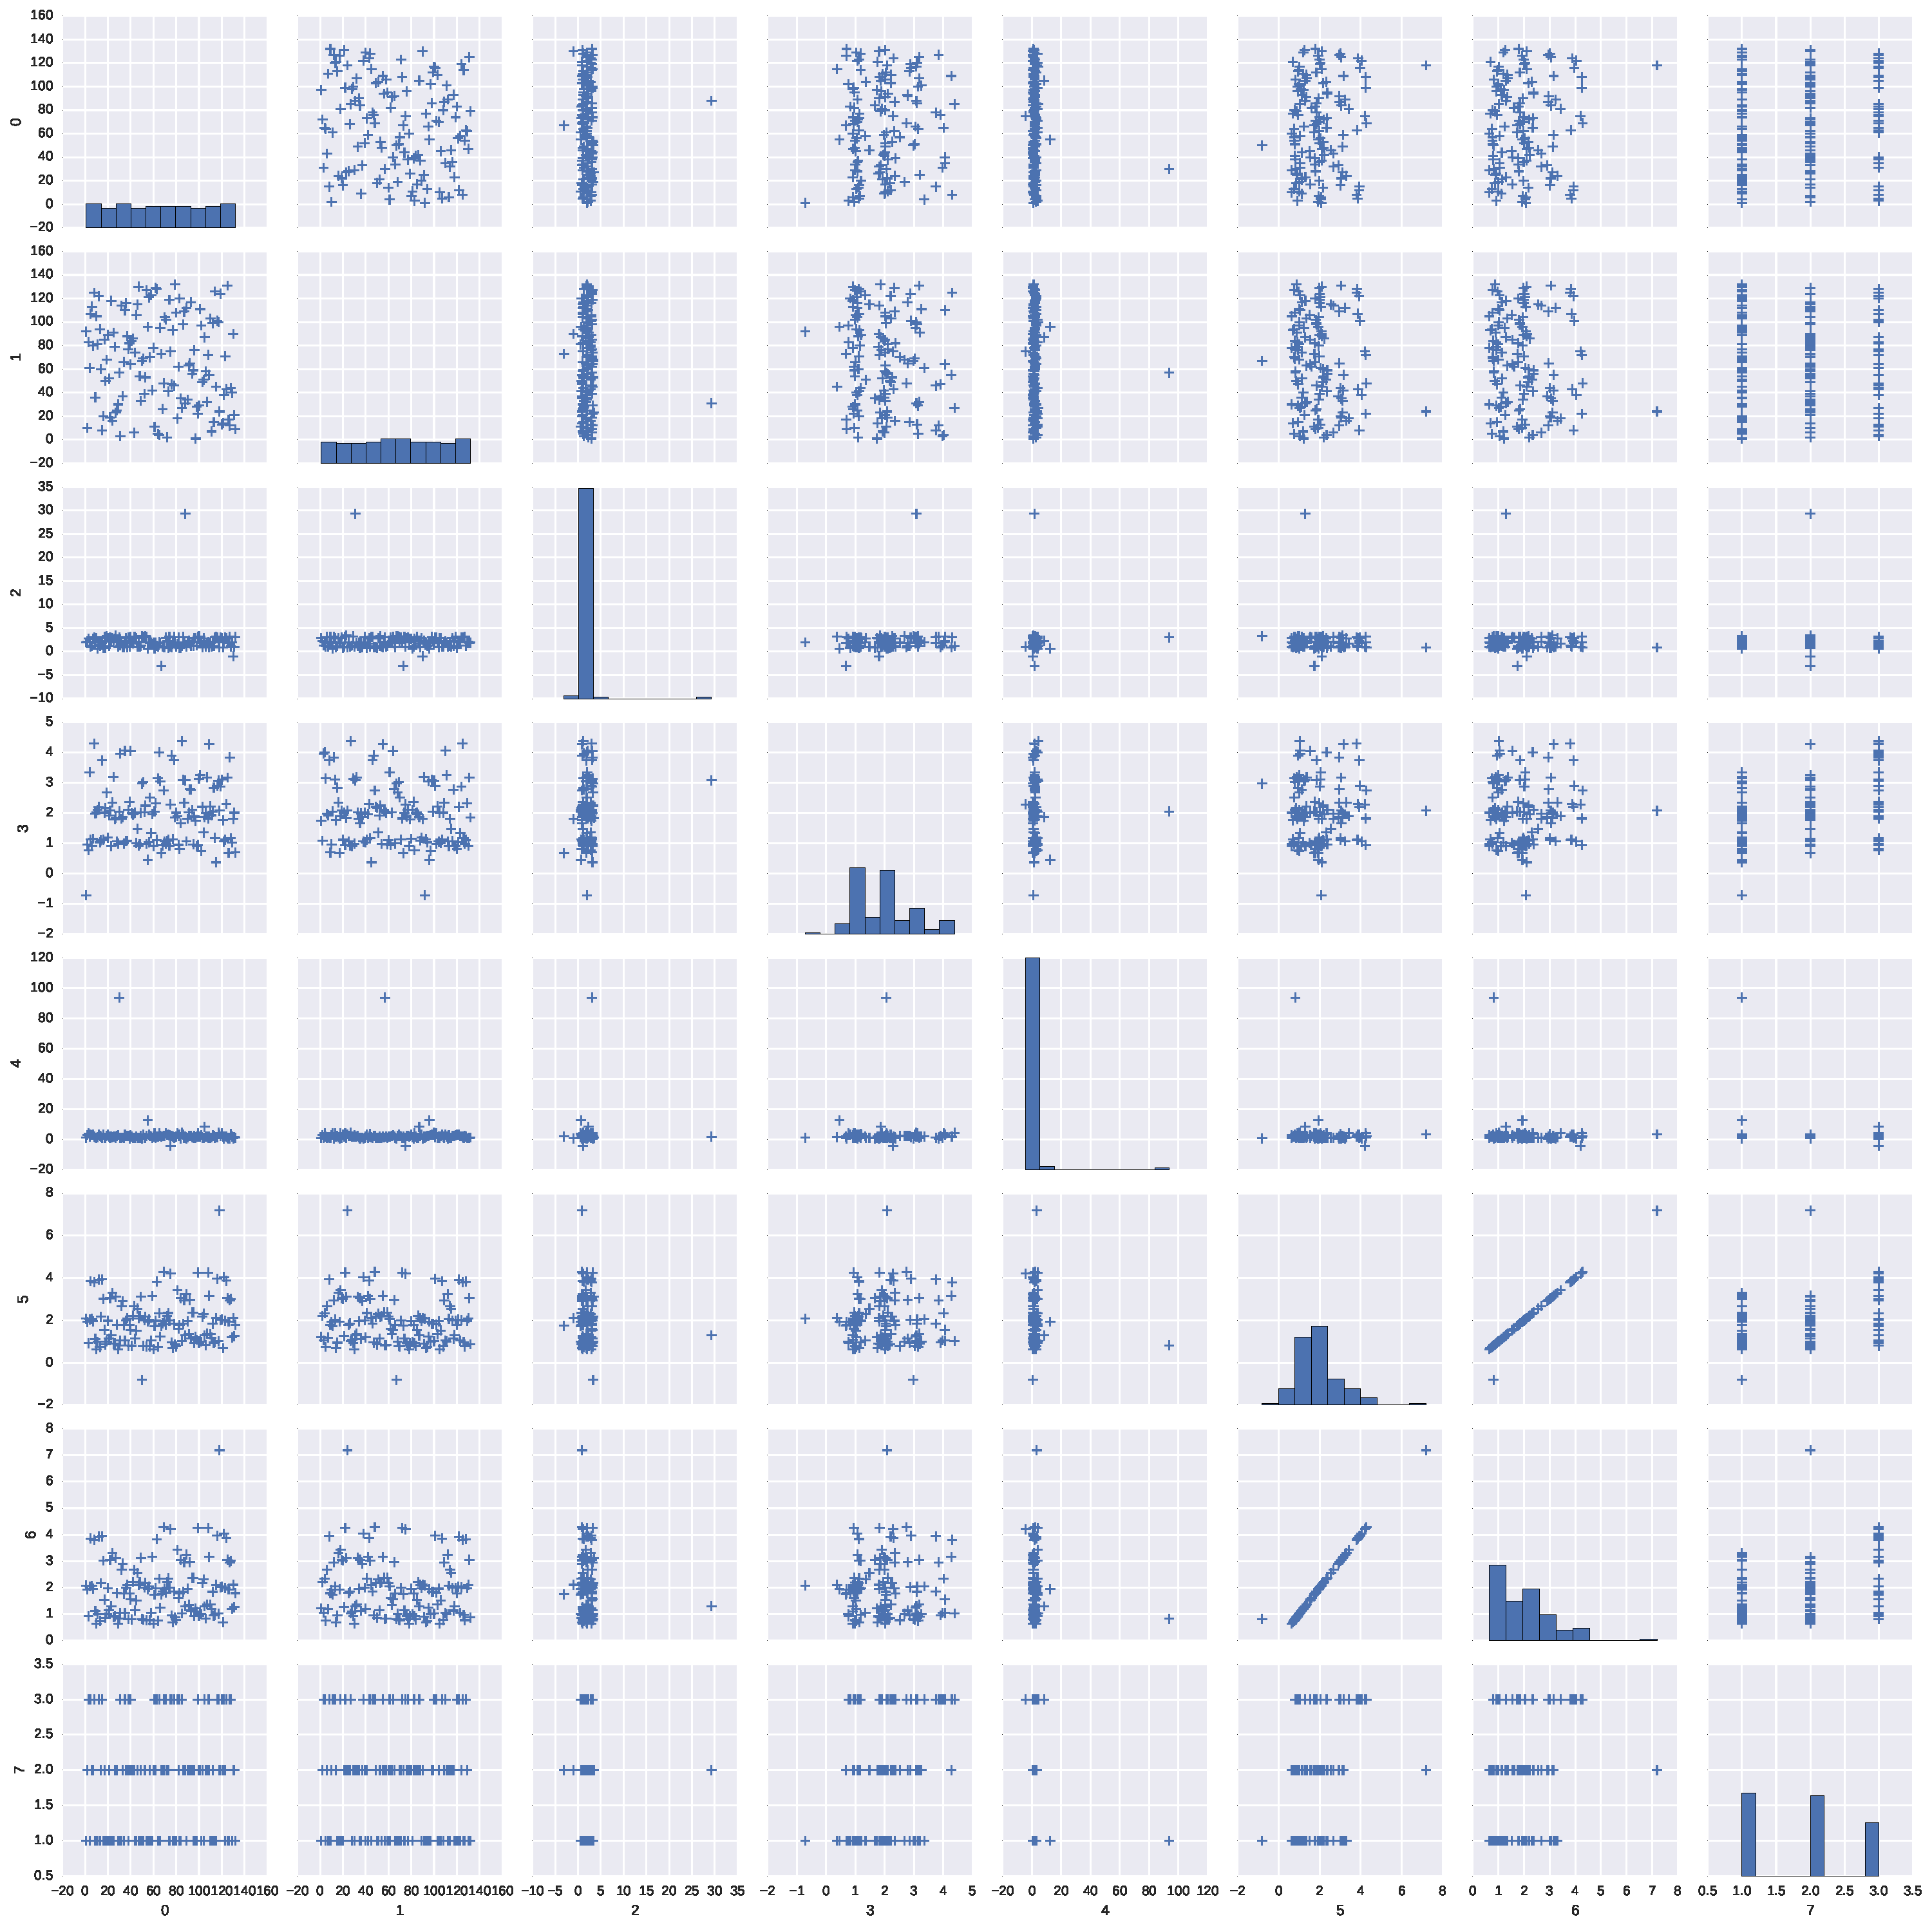
\includegraphics[width=\linewidth]{exercicio3-a.pdf}
		\caption{Antes do pré-processamento.}
		\label{fig:exercicio3-a}
	\end{subfigure}%
	~ 
	\begin{subfigure}[t]{0.49\textwidth}
		\centering
		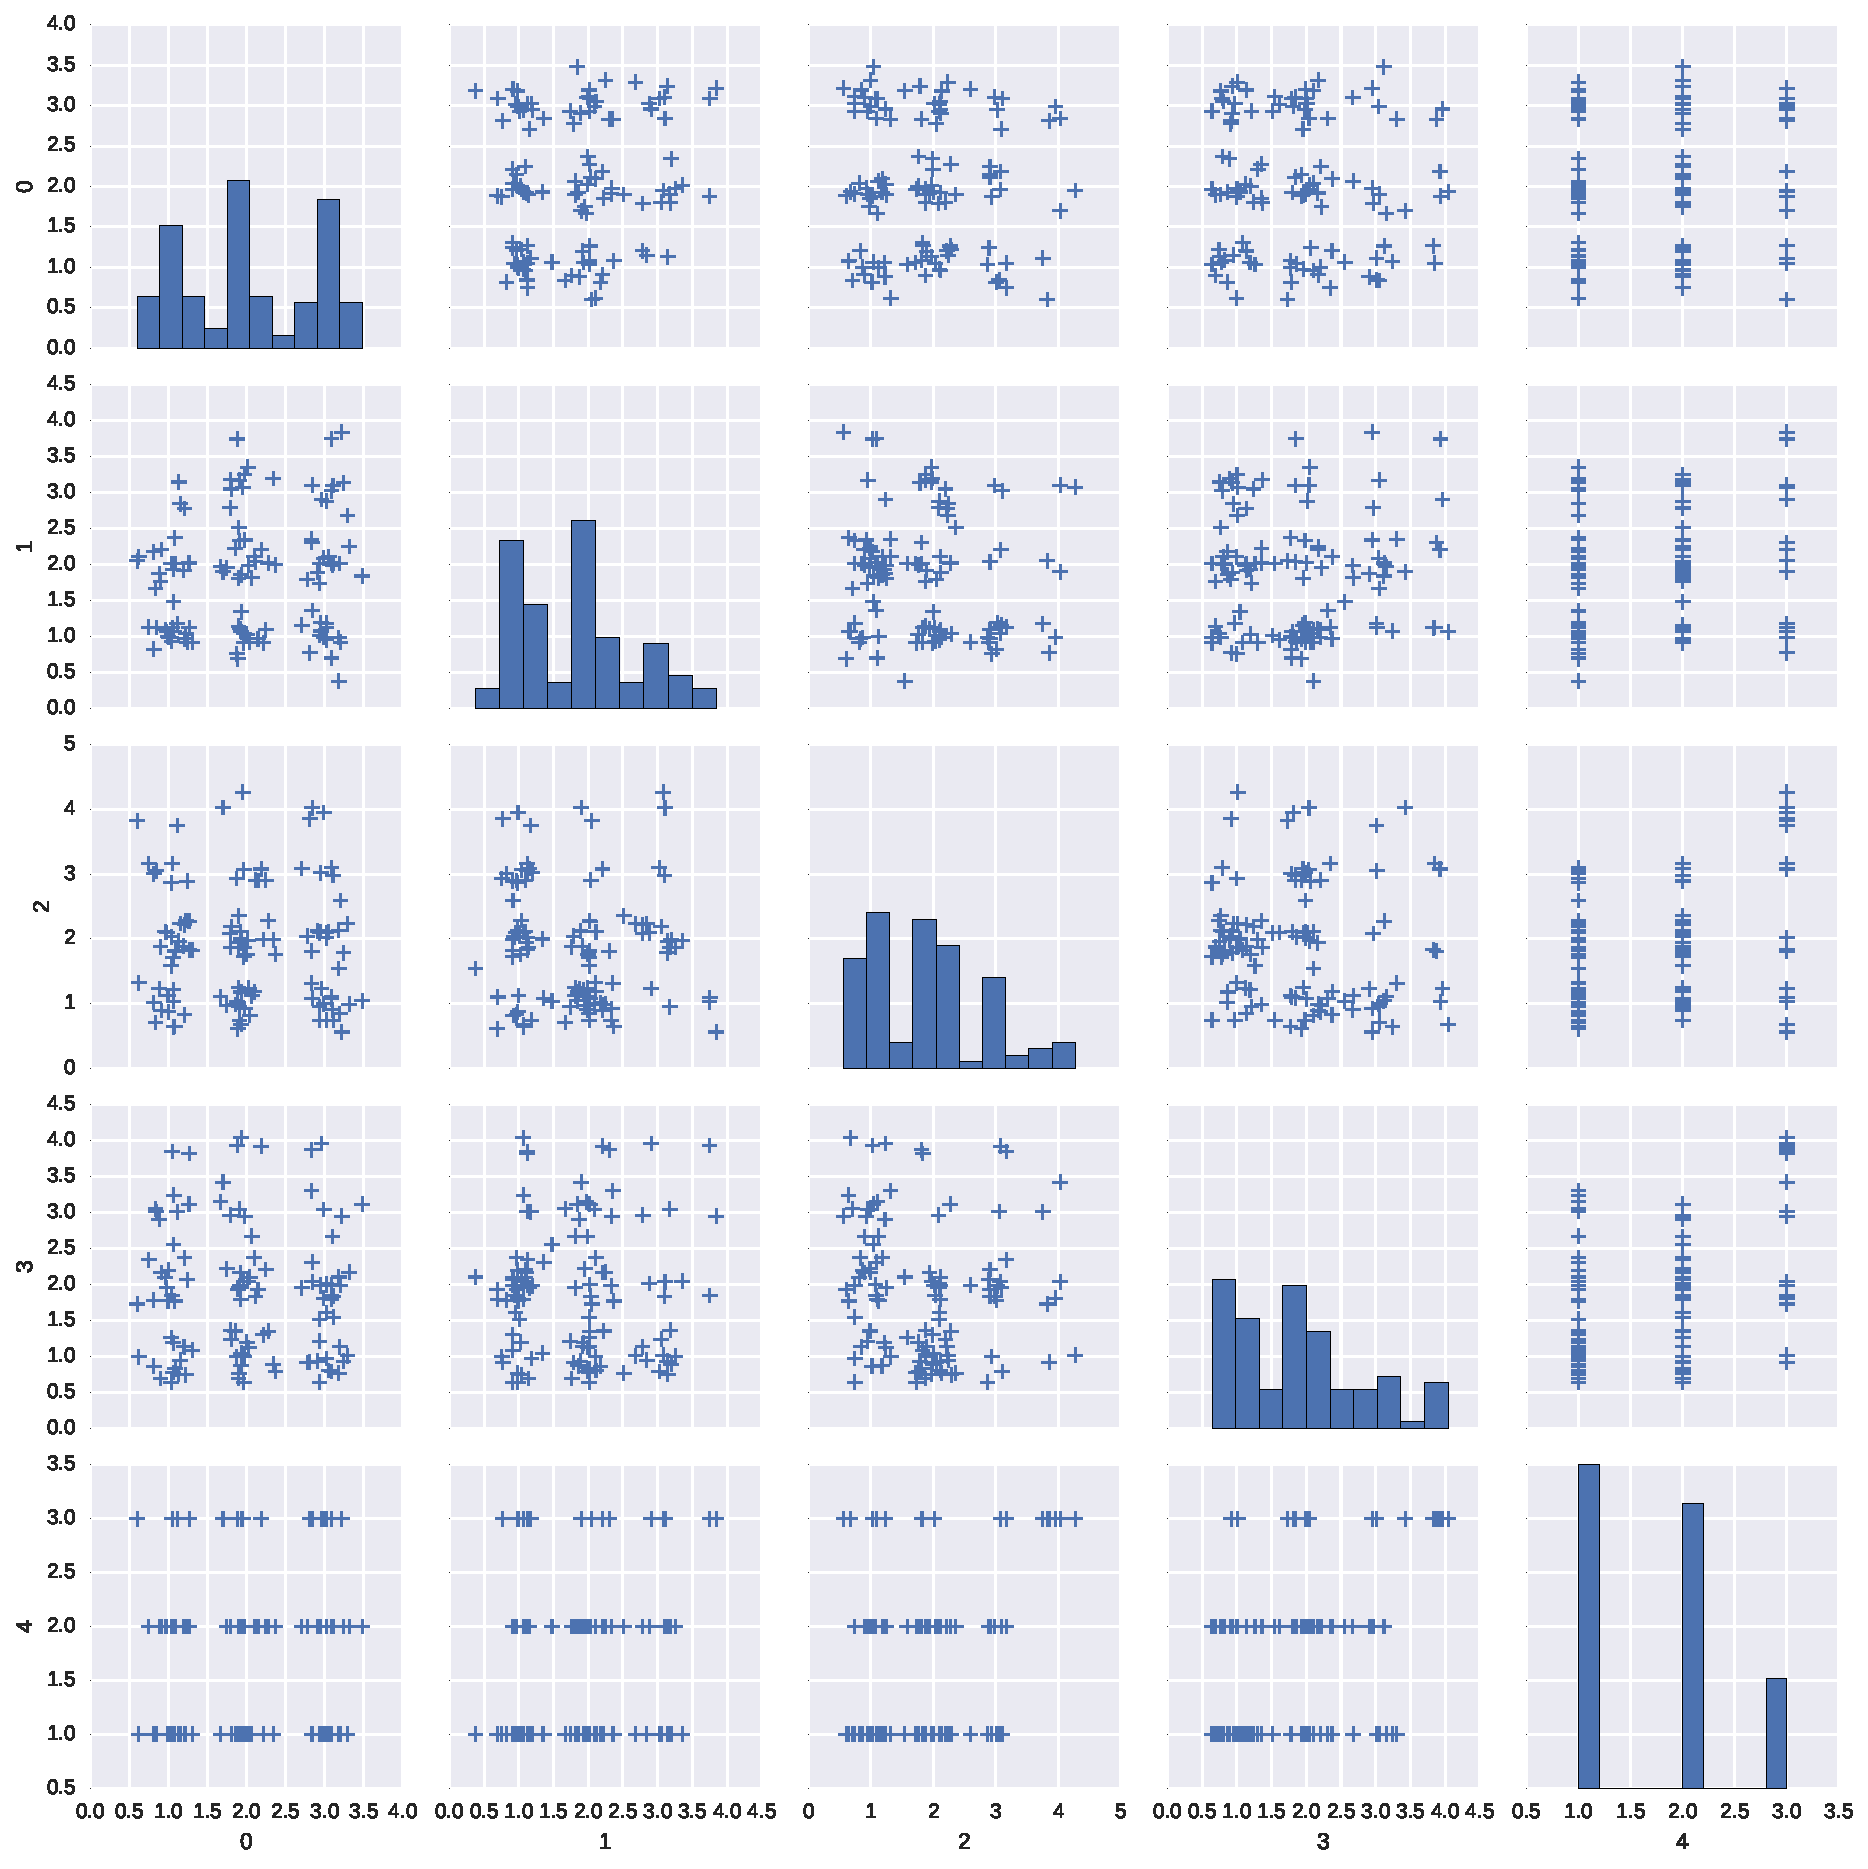
\includegraphics[width=\linewidth]{exercicio3-b.pdf}
		\caption{Depois do pré-processamento.}
		\label{fig:exercicio3-b}
	\end{subfigure}
	\caption{Diferença entre o antes e depois da aplicação das operações de pré-processamento. O último atributo (classe) foi adicionado a visualização somente para verificar que a base é realmente ``nebulosa''.}
\end{figure*}

Após essas operações de pré-processamento, os resultados (acurácia) de classificação no conjunto de teste para as técnicas investigadas foram calculados:

\begin{itemize}
	\item NN: 78.571\%
	\item Rocchio: 46.429\%
\end{itemize}

\paragraph{c)} Compare os resultados obtidos em a) e b). Qual deles retornou o melhor resultado?

Em média, a base de dados pré-processada retornou melhores resultados.

\section{Exercício 4}

Prove que, para uma quantidade de $N$ amostras com entradas $x$ e saídas $t$, as equações

\begin{align*}
w_0 &= \bar{t\vphantom{+1}} - w_1\bar{x\vphantom{+1}} 
& 
w_1 = \frac{\overline{xt\vphantom{+1}}-\bar{x\vphantom{+1}}\bar{t\vphantom{+1}}}{\overline{x^2\vphantom{+1}}-(\bar{x\vphantom{+1}})^2}
\end{align*}

sendo:

\begin{align*}
\bar{a\vphantom{+1}} &= \frac{1}{N} \sum_{k=1}^{N}a_k
\end{align*}

minimizam a função de perda quadrática média L:

\begin{align*}
L &= \frac{1}{N} \sum_{k=1}^{N}(t_k - (w_0 + w_1x_k))^2
\end{align*}

Para minimizar $L$, precisamos de $w_0$ e $w_1$ tal que a função seja minimizada, ou seja:


\begin{align*}
\argmin_{w_0, w_1} \frac{1}{N} \sum_{k=1}^{N}(t_k - (w_0 + w_1x_k))^2
\end{align*}

Podemos abordar esse problema de minimização usando os mínimos quadrados, onde:

\begin{align*}
\frac{\partial L}{\partial w_0} &= 0
& 
\frac{\partial L}{\partial w_1} &= 0
\end{align*}

Derivando em relação a um $w_i$ qualquer, podemos dizer que:

\begin{align*}
\frac{\partial L}{\partial w_i} &= \frac{\partial}{\partial w_i} \left(\frac{1}{N} \sum_{k=1}^{N}(t_k - (w_0 + w_1x_k))^2\right) \\
&= \frac{1}{N} \sum_{k=1}^{N}\left(\frac{\partial}{\partial w_i} \left(t_k - (w_0 + w_1x_k)\right)^2\right)
\end{align*}

Aplicando a Regra da Cadeia, obtemos:

\begin{align*}
\frac{\partial}{\partial w_i} \left(t_k - (w_0 + w_1x_k))^2\right) &= 2(t_k - (w_0 + w_1x_k))(\frac{\partial}{\partial w_i}(t_k - (w_0 + w_1x_k)))
\end{align*}

Logo, podemos dizer que precisamos de um $w_i$ tal que satisfaça a seguinte condição:

\begin{align*}
\frac{1}{N} \sum_{k=1}^{N}\left(2(t_k - (w_0 + w_1x_k))(\frac{\partial}{\partial w_i}(t_k - (w_0 + w_1x_k)))\right) &= 0
\end{align*}

Sabendo que:

\begin{align*}
\frac{\partial}{\partial w_0}(t_k - (w_0 + w_1x_k))) &= -1 & \frac{\partial}{\partial w_1}(t_k - (w_0 + w_1x_k))) &= -x_k
\end{align*}

Podemos concluir, para $w_0$, que:

\begin{align*}
\frac{1}{N} \sum_{k=1}^{N}(2(w_0 + w_1x_k - t_k)) &= 0 \\
w_0 &= \frac{1}{N} \sum_{k=1}^{N}(t_k - w_1x_k)) \\
w_0 &= \bar{t\vphantom{+1}} - w_1\bar{x\vphantom{+1}}
\end{align*}

E, para $w_1$, que:

\begin{align*}
\frac{1}{N} \sum_{k=1}^{N}(2x_k(w_0 + w_1x_k - t_k)) &= 0 \\
w_0\overline{x\vphantom{+1}} + w_1\overline{x^2\vphantom{+1}} - \overline{xt\vphantom{+1}} &= 0
\end{align*}

Substituindo $w_0 = \bar{t\vphantom{+1}} - w_1\bar{x\vphantom{+1}}$, podemos concluir para $w_1$:

\begin{align*}
(\media{t} - w_1\media{x})\overline{x\vphantom{+1}} + w_1\overline{x^2\vphantom{+1}} - \overline{xt\vphantom{+1}} &= 0 \\
\media{x}\media{t} - w_1\big(\media{x}\big)^2 + w_1\overline{x^2\vphantom{+1}} - \overline{xt\vphantom{+1}} &= 0 \\
w_1(\overline{x^2\vphantom{+1}} - \big(\media{x})^2\big) &= \overline{xt\vphantom{+1}} - \media{x}\media{t} \\
w_1 &= \frac{\overline{xt\vphantom{+1}} - \media{x}\media{t}}{\overline{x^2\vphantom{+1}} - \big(\media{x}\big)^2} \\
\end{align*}

\section{Exercício 5}

Para a base de dados Runner (disponibilizada em anexo) obtenha:

\paragraph{a)} A equação linear que se ajusta aos dados e a RMSE;

A equação linear que se ajusta aos dados da base Runner está definida na \autoref{eq:exercicio5-a} e pode ser vista (segmento de reta em vermelho) na \autoref{fig:exercicio5-a}. Essa equação produz um RMSE de 0.220.

\begin{equation}
\label{eq:exercicio5-a}
	f(x) = 36.309 - 0.013x
\end{equation}

\begin{figure}[h]
	\centering
	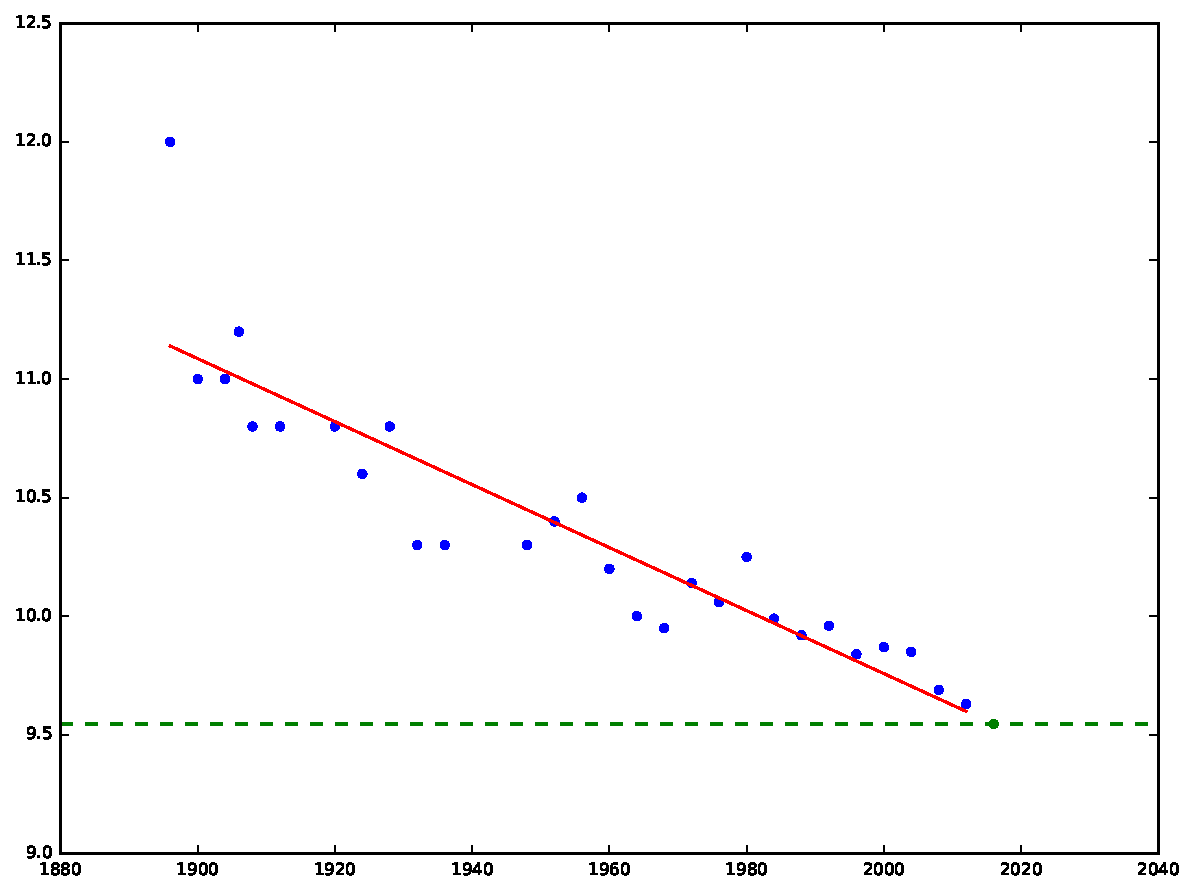
\includegraphics[width=0.5\linewidth]{exercicio5-a.pdf}
	\caption{Base de dados Runner: dados originais (azul) e predição para 2016 (verde). O segmento de reta em vermelho é resultado da regressão linear do dados originais.}
	\label{fig:exercicio5-a}
\end{figure}

\paragraph{b)} Predizer o resultado para o ano de 2016;

Usando a \autoref{eq:exercicio5-a}, com $x=2016$, podemos estimar que em 2016 o tempo será de 9.546 segundos (veja o ponto em verde e segmento de reta verde tracejado na \autoref{fig:exercicio5-a}).

\paragraph{c)} Utilize o teste de hipótese de Kendall para verificar se existe dependência entre os atributos. Realize o teste para 5\% e 1\% de nível de significância;

Inicialmente, é necessário calcular o coeficiente de correlação de Kendall ($\tau$), usando a fórmula apresentada no Slide 58 da Aula 4. Para essa base de dados, temos que $\tau = -0.858$. Em seguida, para utilizar o teste de hipótese, precisamos conhecer os valores de $Z$ para 5\% e 1\% de nível de significância: $Z_{95\%}=1.960$ e $Z_{99\%}=2.576$. Em ambos os níveis de significância (5\% e 1\%), a hipótese nula é rejeitada. Dessa forma, admite-se uma dependência entre as variáveis.

\paragraph{d)} Calcule a correlação entre os dados. Se o módulo da correlação for acima de 0,85
realize o teste de hipótese de Pearson para 5\% e 1\% de nível de significância (teste
bilateral).

Para correlação, será usado o coeficiente de correlação de Pearson ($\rho$), usando a equação disponibilizada no Slide 51 da Aula 4. Para essa base de dados, temos que $\rho = -0.909$. Como o módulo da correlação é maior que o limiar estabelecido, i.e., $|\rho| > 0.85$, o teste de hipótese de Pearson é realizado. O teste de hipótese foi realizado para dois níveis de significância (5\% e 1\%), onde verificou-se que a hipótese nula foi rejeitada em ambos. Então, admite-se a possibilidade de haver dependência entre as variáveis.

\section{Exercício 6}
Para a base de dados Polinômio (disponibilizada em anexo), faça:

\paragraph{a)} Divida aleatoriamente a base de dados em duas partes: treino, como 70\% das amostras, e teste, com 30\%. Use a parte de treino para estimar um modelo linear que melhor se ajusta aos dados, sendo a entrada do modelo a primeira coluna e a saída a segunda coluna. Informe os parâmetros do modelo encontrado e obtenha os valores de RMSE e MAPE sobre o conjunto de treino e teste. Mostre um gráfico do modelo estimado e dos pontos da base de dados. O modelo conseguiu se ajustar bem aos dados? Por quê?

Os dados foram divididos aleatoriamente usando uma seed (2017) para garantir a reprodução dos resultados. Das 170 amostras iniciais, 119 ficaram no conjunto de treino e as outras 51 no conjunto de teste. O modelo linear definido pela \autoref{eq:exercicio6-a} é o que melhor se ajusta aos dados de treino.

\begin{equation}
\label{eq:exercicio6-a}
f(x) = -299.749 + 106.110x
\end{equation}

Nos dados de treino, esse modelo alcançou $\mathrm{RMSE} = 230.002$ e $\mathrm{MAPE} = 411750.145$. No conjunto de teste, o modelo alcançou $\mathrm{RMSE} = 194.241$ e $\mathrm{MAPE} = 2409.121$. Como pode ser visto na \autoref{fig:exercicio6-a} (gráfico do modelo estimado e dos pontos da base de dados), o modelo não conseguiu se ajustar bem aos dados, pois os dados não obedecem uma função linear.

\begin{figure}[h]
	\centering
	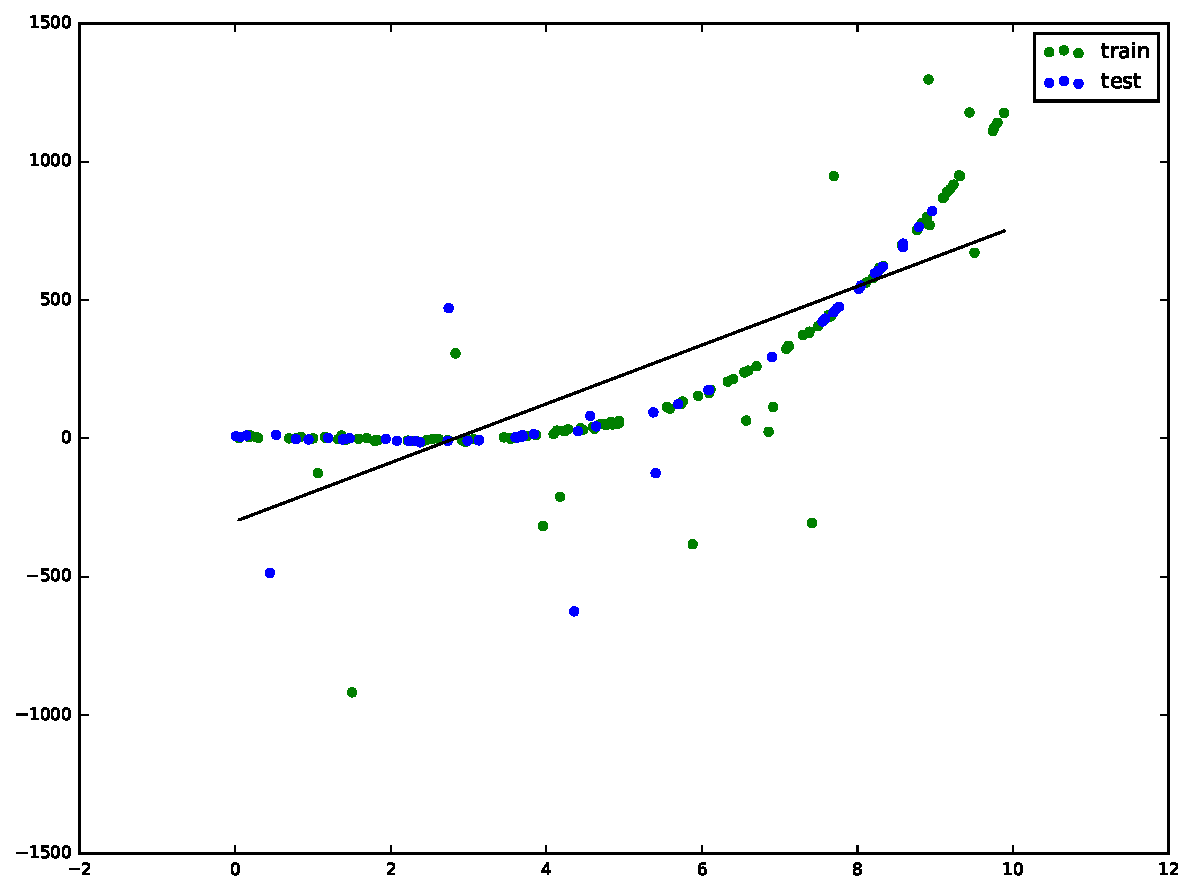
\includegraphics[width=0.5\linewidth]{exercicio6-a.pdf}
	\caption{Modelo linear (preto) ajustado com os dados do conjunto de treino (verde).}
	\label{fig:exercicio6-a}
\end{figure}

\paragraph{b)} Estimar o modelo polinomial que melhor se ajusta aos dados usando os dados de treinamento. Informe os parâmetros do modelo encontrado. Use os fatores de determinação de complexidade do modelo para auxiliar a encontrar o modelo. Obtenha os valores RMSE e MAPE do modelo obtido sobre os dados de treino e teste. Mostre um gráfico com o novo modelo. O modelo conseguiu se ajustar melhor aos dados? Por quê?

Para encontrar um modelo polinominal $f(x) = a_0 + a_1x + a_2x_2 + \dots + a_{n-1}x^{n-1} + a_nx^n$, precisamos encontrar um $n$ tal que o polinômio resultante seja o que melhor se ajuste aos dados. Para isso, o conjunto de treino inicial foi dividido em 2 outros conjuntos: treino e validação (70\% e 30\% dos dados de treino inicial, respectivamente). Essa divisão entre conjunto de treino e validação também foi feita aleatoriamente. Com esses 2 conjuntos, foi realizada uma busca entre os modelos polinomiais variando $n$ entre 1 e 10, usando o coeficiente de determinação (R$^2$) para escolher qual foi o melhor modelo. Como pode ser visto na \autoref{fig:exercicio6-b-tuning}, o melhor modelo polinomial alcançou R$^2 = 0.951$ com $n=3$.

\begin{figure}[h]
	\centering
	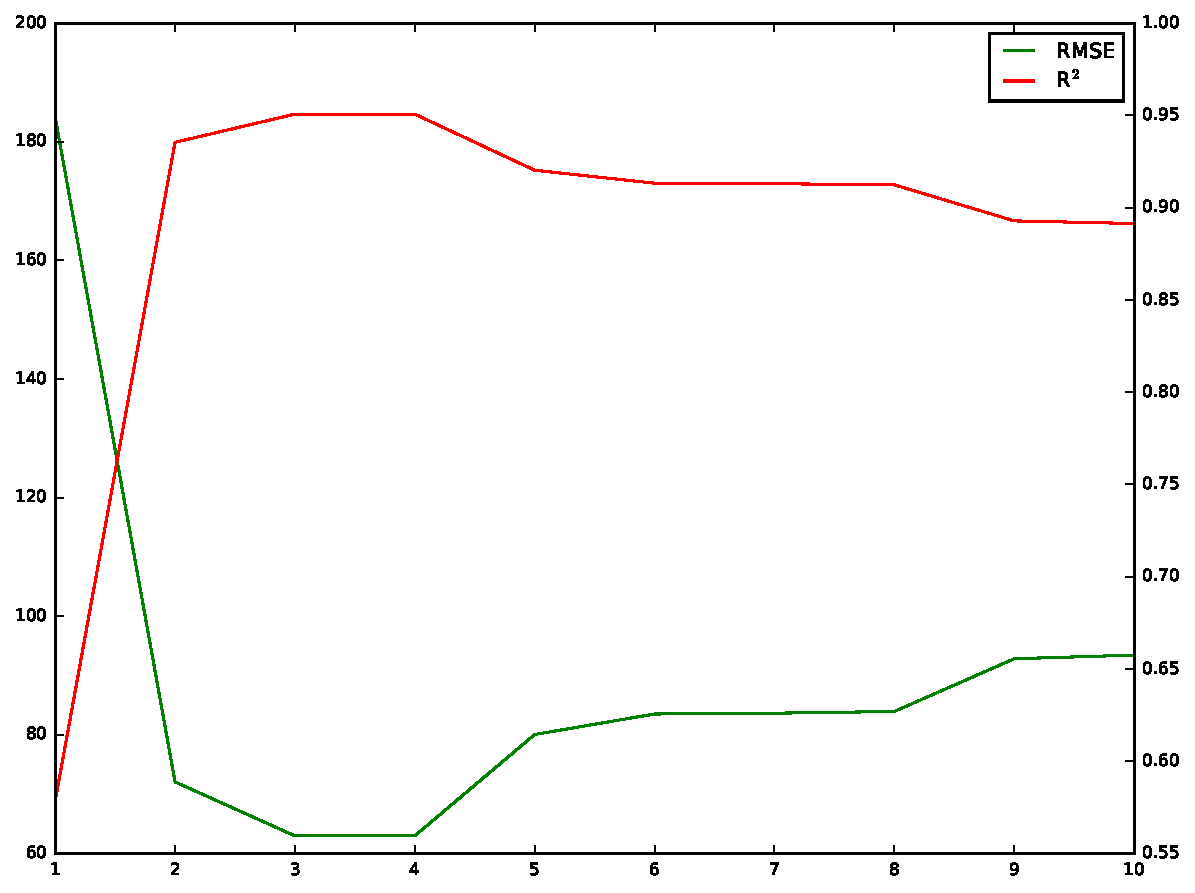
\includegraphics[width=0.5\linewidth]{exercicio6-b-tuning.pdf}
	\caption{Ajuste do parâmetro $n$ que define o grau do polinômino.}
	\label{fig:exercicio6-b-tuning}
\end{figure}

Então, o modelo polinomial ($n=3$) definido pela \autoref{eq:exercicio6-b} foi treinado no conjunto de treino inicial e avaliado conforme solicitado.

\begin{equation}
\label{eq:exercicio6-b}
f(x) = -25.274 + 14.276x - 12.316x^2 + 2.372x^3
\end{equation}

Nos dados de treino, esse modelo alcançou $\mathrm{RMSE} = 147.596$ e $\mathrm{MAPE} = 37876.289$. No conjunto de teste, o modelo alcançou $\mathrm{RMSE} = 134.684$ e $\mathrm{MAPE} = 426.564$. Como pode ser visto na \autoref{fig:exercicio6-b} (gráfico do modelo estimado e dos pontos da base de dados), o modelo conseguiu se ajustar melhor aos dados em comparação com o modelo linear, com R$^2 = 0.852$ nos dados de treino inicial e R$^2 = 0.800$ nos dados de teste.

\begin{figure}[h]
	\centering
	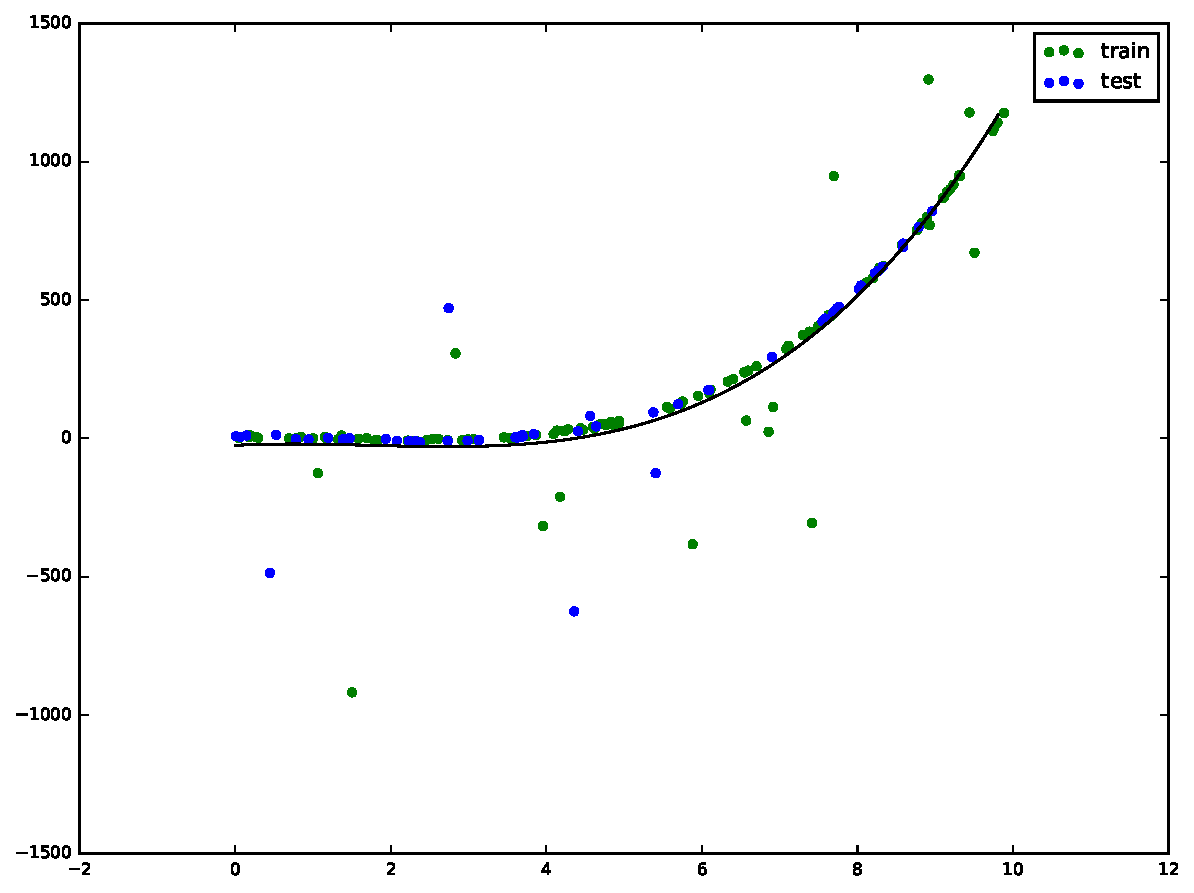
\includegraphics[width=0.5\linewidth]{exercicio6-b.pdf}
	\caption{Modelo polinomial (preto) ajustado com os dados do conjunto de treino (verde).}
	\label{fig:exercicio6-b}
\end{figure}

\paragraph{c)} Utilize o método de Ransac sobre os dados de treinamento para remover os outliers e obter o modelo polinomial. Informe os parâmetros do modelo encontrado. Obtenha o RMSE e MAPE do modelo obtido sobre os dados de treino e teste. Mostre um gráfico com o novo modelo. O Ransac conseguiu ajustar melhor o modelo aos dados?

Para aplicar o RANSAC são necessários diversos parâmetros. Seguindo a nomenclatura utilizada no Slide 42 da Aula 4, dois dos parâmetros ($T$ e $L$) podem ser calculados de acordo com as fórmulas apresentadas nos Slides 43 e 45 da Aula 4, respectivamente. Para os cálculos, foram usados os valores padrões de $p=0.99$ e $\epsilon=0.2$. Aplicando as fórmulas, temos $T=95$ e $L = 165200$. O $\tau$ também poderia ser calculado, mas foi empiracamente escolhido ($\tau=10$). O número de amostras a serem escolhidas aleatoriamente foi definido empiricamente como $s = \frac{T}{2}$, onde $\frac{T}{2} = 47$. Com esses parâmetros, o RANSAC precisou de 274 iterações para selecionar um modelo (definido pela \autoref{eq:exercicio6-c}) com 102 \textit{inliers}, que é maior do que $T$.

\begin{equation}
\label{eq:exercicio6-c}
f(x) = -1.449 + 6.673x - 9.151x^2 + 2.072x^3
\end{equation}

Nos dados de treino, esse modelo alcançou $\mathrm{RMSE} = 149.476$ e $\mathrm{MAPE} = 4219.095$. No conjunto de teste, o modelo alcançou $\mathrm{RMSE} = 136.196$ e $\mathrm{MAPE} = 55.748$. Como pode ser visto na \autoref{fig:exercicio6-c}, o modelo parece ter se ajustado melhor aos dados em comparação com modelo polinomial anterior (encontrado no item \textit{b}). Desconsiderando os outliers (de acordo com o $\tau$ definido), esse novo modelo alcançou $\mathrm{RMSE} = 4.008$ no treino. É importante notar que a métrica MAPE é muito influenciada pelos erros nos valores próximos de zero.

\begin{figure}[h]
	\centering
	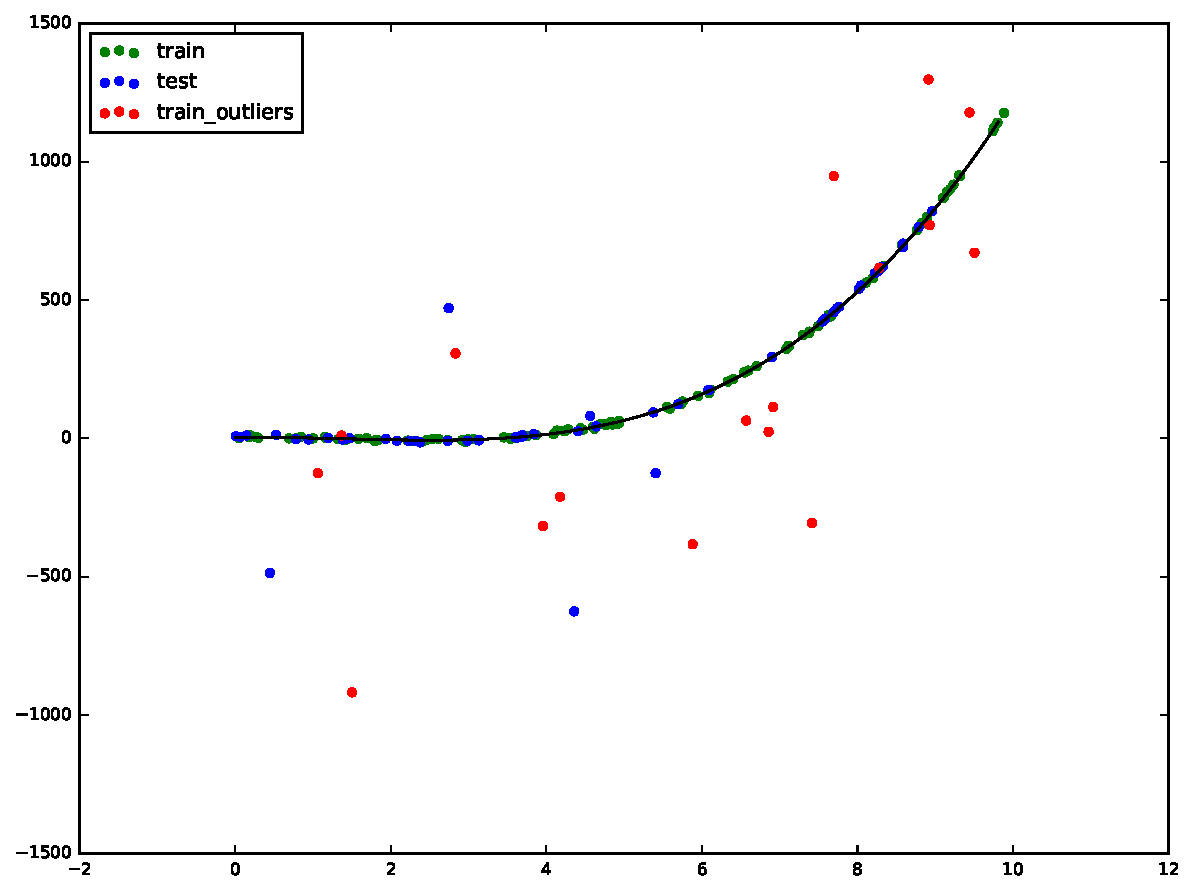
\includegraphics[width=0.5\linewidth]{exercicio6-c.pdf}
	\caption{Modelo polinomial (preto) ajustado com os dados do conjunto de treino (verde) sem outliers (vermelho). Os outliers foram identificados com o uso do RANSAC.}
	\label{fig:exercicio6-c}
\end{figure}


\section{Exercício 7}

Explique o dilema entre bias e variância e o seu relacionamento com underfitting e
overfitting.

Seja $f(x)$ um modelo (por exemplo, uma rede neural treinada), podemos dizer que o erro esperado de $f(x)$ para uma amostra $x$ não vista no treino pode ser decomposto em função do bias e da variância, como pode ser visto no Slide 36 da Aula 4. Desse modo, a complexidade de um modelo está atrelada ao bias e a variância de tal forma que modelos de baixa complexidade possuem erro da variância baixo e erro do bias alto (fazendo com que o modelo não consiga se ajustar ao problema -- \textit{underfitting}) e modelos de alta complexidade possuem erro de variância alto e erro do bias baixo (fazendo com que o modelo se ajuste demais aos dados de treino -- \textit{overfitting}). O \textit{tradeoff} pode ser claramente observado no gráfico apresentado no Slide 38 da Aula 4. O dilema consiste em encontrar um modelo equilibrado em relação aos erros do bias e da variância.

\section{Exercício 8}

Para a figura abaixo, obtenha o diagrama de Voronoi das amostras quadrado, triângulo
e losango para as métricas de:

\paragraph{a)} Distância Euclidiana;

Veja o diagrama de Voronoi na \autoref{fig:exercicio8-a}.

\begin{figure}[h]
	\centering
	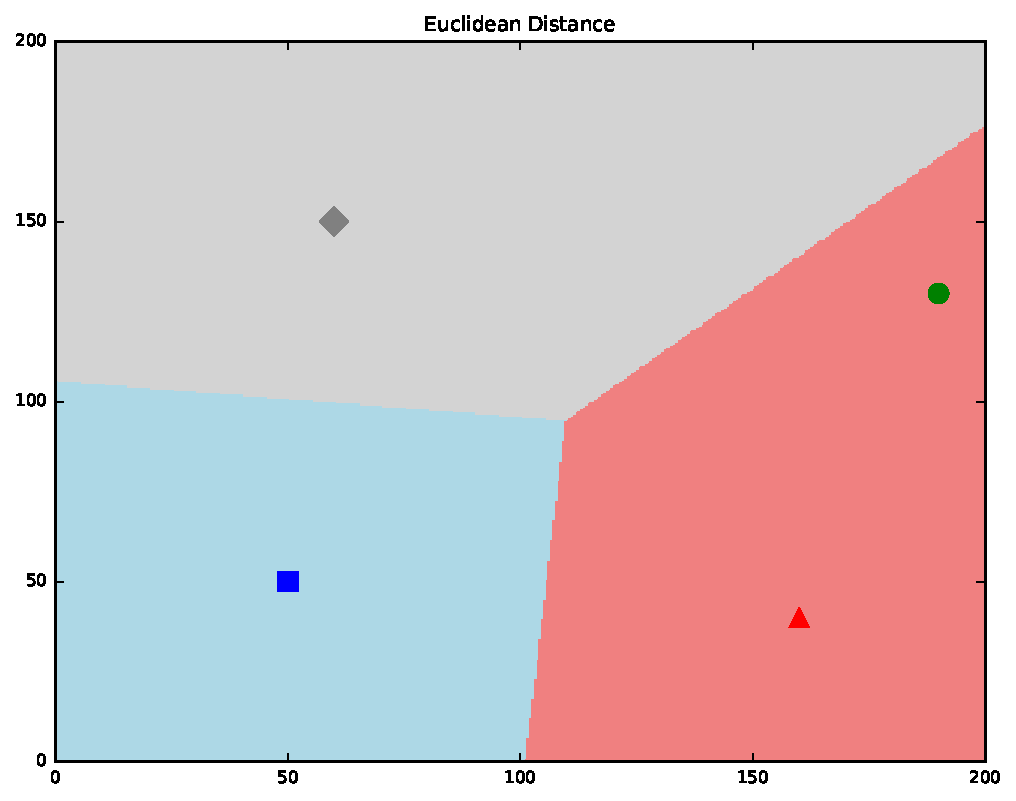
\includegraphics[width=0.5\linewidth]{exercicio8-a.pdf}
	\caption{Diagrama de Voronoi usando a Distância Euclidiana como métrica.}
	\label{fig:exercicio8-a}
\end{figure}

\paragraph{b)} Similaridade Cosseno;

Veja o diagrama de Voronoi na \autoref{fig:exercicio8-b}.

\begin{figure}[h]
	\centering
	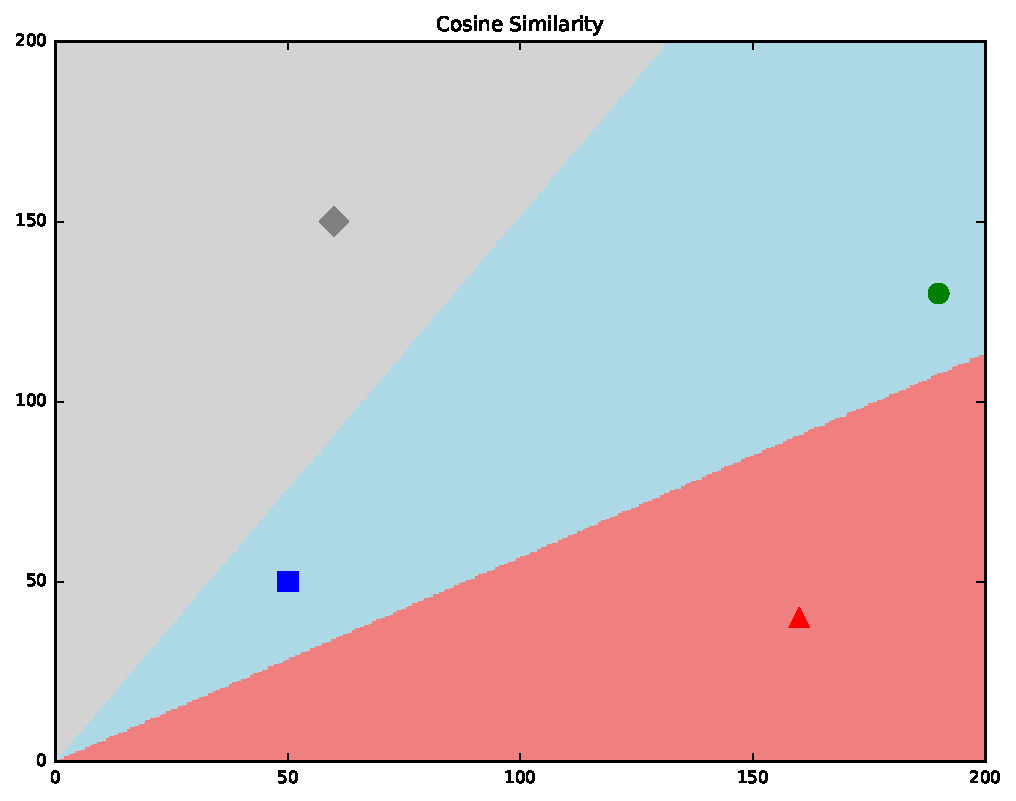
\includegraphics[width=0.5\linewidth]{exercicio8-b.pdf}
	\caption{Diagrama de Voronoi usando a Similaridade de Cosseno como métrica.}
	\label{fig:exercicio8-b}
\end{figure}

\paragraph{c)} Obtenha a classe (quadrado, triângulo ou losango) da amostra círculo para um
classificador NN, se for usada a métrica de Distância Euclidiana e a Similaridade Cosseno.

A classe da amostra círculo, usando um classificador NN, será predita como triângulo (veja a região em vermelho na \autoref{fig:exercicio8-a}) se for usada a métrica de Distância Euclidiana ou quadrado (veja a região em azul na \autoref{fig:exercicio8-b}) se for usada a métrica de Similaridade Cosseno.

\section{Exercício 9}

Realize a classificação da base de dados \texttt{Car Evaluation} (disponível em \url{http://archive.ics.uci.edu/ml/}) usando o kNN. Realize 3-fold cross validation e, para cada rodada, use dois folds para a parte de calibração e um fold para teste. Na parte de calibração o treinamento deve ser realizado usando um fold e a validação do valor de k deve ser realizado usando o outro fold. A calibração deve ser realizada de forma a maximizar a acurácia. Expresse os resultados em forma de acurácia média, macroprecision médio, macrorecall médio e tabela de contingência médio (dado em porcentagem).

A base de dados \texttt{Car Evaluation} consiste em 1728 amostras com 6 atributos e 1 classe. Inicialmente, a base de dados foi convertida dos valores categóricos para numéricos. Como os atributos parecem possuir uma ordem, i.e., o mapeamento categoria $\rightarrow$ número foi feito de modo a preservar essa relação de ordem. Além dessa conversão, os valores numéricos sequenciais foram normalizados por atributo para média zero e variância unitária. Essa normalização apresentou melhores resultados durante a calibração. Depois, os dados foram embaralhados para realizar a separação em 3 folds. Cada fold ficou com 576 amostras. Conforme orientado, para o $k$-ésimo fold, o fold $k$ foi usado na validação, o fold $(k+1) \mathbin{\%} 3$ foi usado no treino e o fold $(k+2) \mathbin{\%} 3$ foi usado no teste, onde $A\mathbin{\%}B$ representa o resto da divisão de $A$ por $B$. Dois fatores foram ajustados durante a calibração: o valor do $k$ e a métrica de distância. Foram testados valores de 1 até 10 para o $k$ e 3 métricas foram avaliadas durante a calibração: Distância de Manhattan, Distância Euclidiana e Similaridade de Cosseno. O processo de calibração para cada fold pode ser visto na \autoref{fig:exercicio9}.

\begin{figure*}[t!]
	\centering
	\begin{subfigure}[t]{0.32\textwidth}
		\centering
		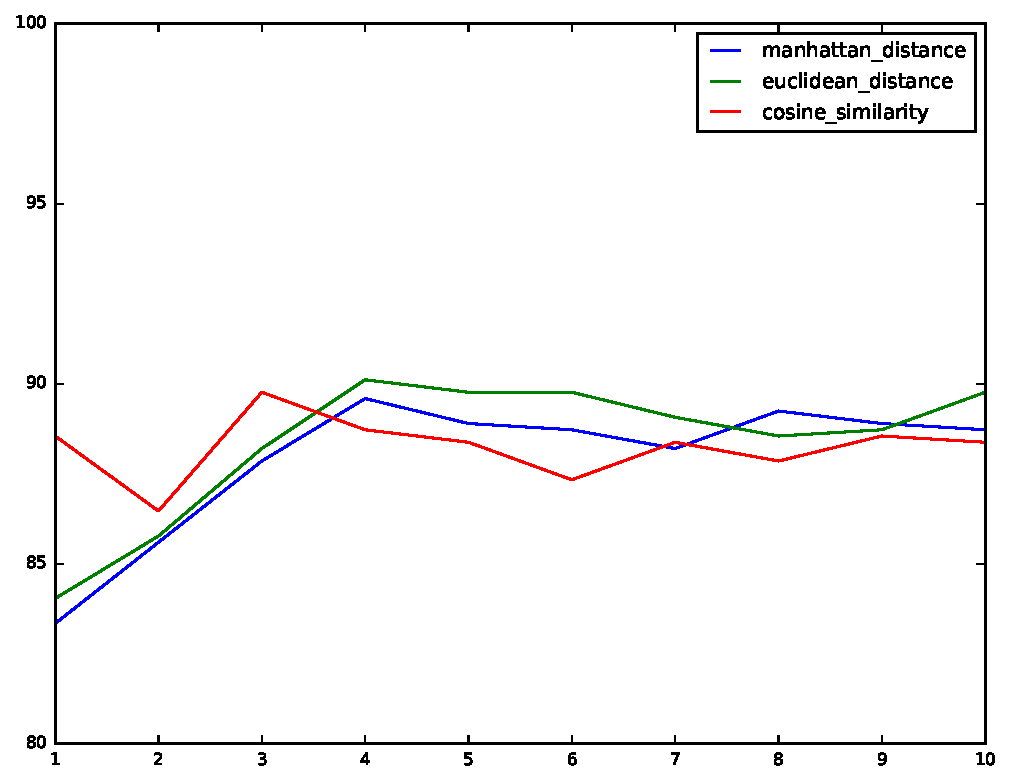
\includegraphics[width=\linewidth]{exercicio9-fold-1.pdf}
		\caption{Fold 1. Melhor configuração: Distância Euclidiana com $k=4$.}
	\end{subfigure}%
	~ 
	\begin{subfigure}[t]{0.32\textwidth}
		\centering
		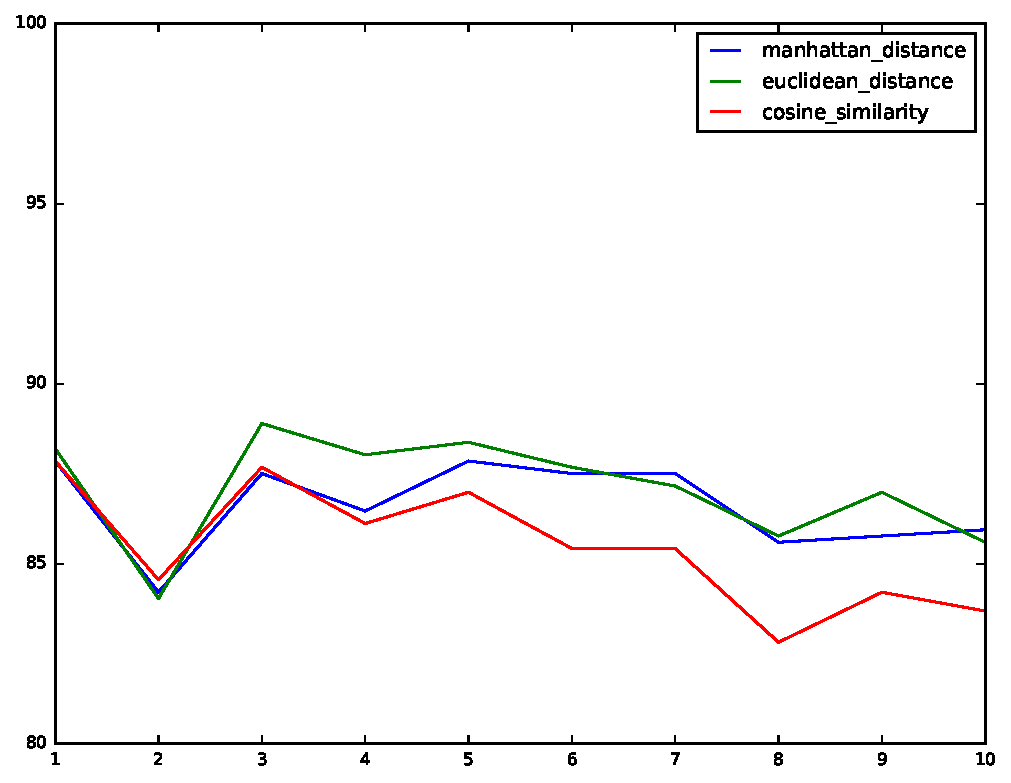
\includegraphics[width=\linewidth]{exercicio9-fold-2.pdf}
		\caption{Fold 2. Melhor configuração: Distância Euclidiana com $k=3$.}
	\end{subfigure}
	~ 
	\begin{subfigure}[t]{0.32\textwidth}
		\centering
		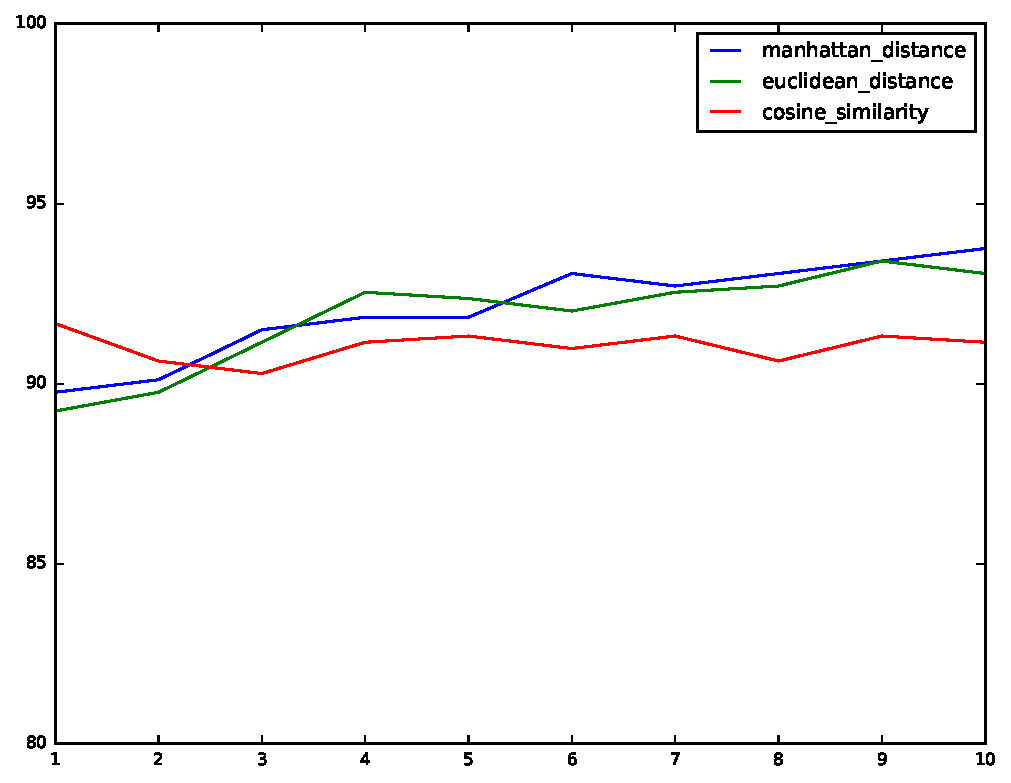
\includegraphics[width=\linewidth]{exercicio9-fold-3.pdf}
		\caption{Fold 3. Melhor configuração: Dist. de Manhattan com $k=10$.}
	\end{subfigure}
	\caption{Calibração do kNN para cada um dos 3 folds na base de dados \texttt{Car Evaluation}.}
	\label{fig:exercicio9}
\end{figure*}

A melhor configuração (maximizando a acurácia no fold de validação) de cada um dos 3 folds foi avaliada no respectivo fold de teste para calcular as métricas de interesse. Os resultados foram:

\begin{itemize}
	\item Acurácia média: 89.988\%
	\item Macro-precision médio: 85.148\%
	\item Macro-recall médio: 68.217\%
	\item Tabela de Contingência média (em \%): \autoref{tab:exercicio9}
\end{itemize}

\begin{table}[]
	\centering
	\caption{Tabela de Contingência Média (em \%)}
	\label{tab:exercicio9}
	\begin{tabular}{@{}l|cccc@{}}
		& 1      & 2      & 3      & 4      \\ \midrule
		1. unacc & \textbf{93.815} & 5.383  & 0.725  & 0.077  \\
		2. acc   & 7.042  & \textbf{79.228} & 8.877  & 4.851  \\
		3. good  & 0.000  & 9.722  & \textbf{77.778} & 12.500 \\
		4. vgood & 0.000  & 1.961  & 8.269  & \textbf{89.770}
	\end{tabular}
\end{table}

\section{Exercício 10}

Usando as técnicas de seleção de características SFS e SBS sobre a base de dados Wine (disponível em \url{http://archive.ics.uci.edu/ml/}), faça:

\paragraph{a)} Divida a base de dados em três partes de forma estratificada. Selecione 5 atributos usando uma parte da base de dados como treinamento e valide os atributos sobre uma outra parte usando a métrica acurácia. Após determinar os 5 atributos, obtenha a acurácia sobre a terceira parte, usando as duas partes anteriores como treinamento. Use o classificador Vizinho mais Próximo nesta tarefa. Quais foram os atributos selecionados?

Antes de aplicar as técnicas de seleção de características, a base de dados foi normalizada para média zero e variância unitária. Para o Vizinho mais Próximo, usando Distância Euclidiana, os índices dos 5 atributos\footnote{O nome de cada um dos 13 atributos da base de dados Wine está disponível em \url{http://archive.ics.uci.edu/ml/machine-learning-databases/wine/wine.names}.} selecionados por cada uma das duas técnicas foram:

\begin{itemize}
	\item SFS (acurácia no teste: 94.828\%): 1, 7, 10, 11, 13
	\item SBS (acurácia no teste: 93.103\%): 1, 7, 10, 12, 13
\end{itemize}

\paragraph{b)} Realize o mesmo procedimento, mas agora selecionando 10 atributos;

Cada uma das técnicas selecionou 10 atributos com os seguintes índices:

\begin{itemize}
	\item SFS (acurácia no teste: 98.276\%): 1, 2, 4, 5, 6, 7, 8, 10, 11, 13
	\item SBS (acurácia no teste: 98.276\%): 1, 5, 6, 7, 8, 9, 10, 11, 12, 13
\end{itemize}

\paragraph{c)} Realize o mesmo procedimento de a) e b), mas agora selecionando os atributos usando duas partes para treinamento e validando sobre as mesmas duas partes. Após determinar os atributos, obtenha a acurácia sobre a terceira parte. A acurácia sobre a terceira parte foi melhor, igual ou pior do que as obtidas nas letras a) e b). Por quê?

Os experimentos \textit{a)} e \textit{b)} foram refeitos treinando e validando sobre as mesmas duas partes. Os resultados foram:

\begin{itemize}
	\item 5 atributos:
		\begin{itemize}
			\item SFS (acurácia no teste: 79.310\%): 1, 2, 3, 4, 5
			\item SBS (acurácia no teste: 94.828\%): 9, 10, 11, 12, 13
		\end{itemize}
	\item 10 atributos:
		\begin{itemize}
			\item SFS (acurácia no teste: 94.828\%): 1, 2, 3, 4, 5, 6, 7, 8, 9, 10
			\item SBS (acurácia no teste: 96.552\%): 4, 5, 6, 7, 8, 9, 10, 11, 12, 13
		\end{itemize}
\end{itemize}

Como pode ser observado, os resultados ficaram, na média, piores do que os alcançados nas letras \textit{a)} e \textit{b)}. Caso a normalização não seja aplicada nos dados, a diferença entre os experimentos fica ainda maior. Essa piora se deve, parcialmente, ao fato de que o classificador usado (Vizinho mais Próximo) alcança 100\% de acurácia quando treinado e validado nos mesmos dados. Esse fato faz com que o processo de seleção de características não seja realístico, podendo selecionar ou descartar qualquer característica sem impacto na métrica de interesse durante a calibração.

\section*{Instruções para usar os scripts}

O código-fonte enviado foi desenvolvido em Python. Esse código foi testado tanto no Linux (Ubuntu 14.04) quanto no Windows 10. Para rodar os scripts dos exercícios, é necessário ter Python 2.7 ou Python 3.x instalado na sua máquina e algumas dependências. Para instalar as dependências, basta rodar o comando abaixo na raiz do repositório:

\begin{verbatim}
	$ pip install -r lista1/requirements.txt
\end{verbatim}

Para executar o script de um exercicio em específico (por exemplo, o exercício 1), basta executar:

\begin{verbatim}
	$ cd lista1/scripts
	$ python lista1.py --exercicio=1
\end{verbatim}

Ou então, se preferir, você pode executar o script diretamente. Por exemplo:

\begin{verbatim}
	$ cd lista1/scripts
	$ python exercicio1.py
\end{verbatim}

As bases de dados Iris, Car Evaluation e Wine serão baixadas automaticamente nas questões em que foram usadas. Todas as bases de dados estão armazenadas na pasta \texttt{data}. Ao executar os scripts, os gráficos que estão neste relatório serão exibidos e salvos na pasta \texttt{output}. O codigo-fonte desse relatório (em \LaTeX) também se encontra na pasta \texttt{report}. Para garantir a reprodutibilidade dos resultados e gráficos, foi usado como seed o valor \texttt{2017} definido no arquivo \texttt{scripts/constants.py}.

\end{document}
